
\Chapter{Evaluation}

As stated in previous chapters, the Learning Analytics Software was created with two principal objectives. The first is to monitor the performance of the students in different levels: individual, per quiz and per group. The second is to ease the understanding of the items in online quizzes in order to improve the design of future quiz items \footnote{The second objective is focused on the understanding of the Item Response Theory.}. These two objectives were evaluated with a focus group that consisted of 3 persons working with online quizzes and interested in learning analytics topics. 

The general structure of the focus group consists of two big sections of 30 minutes each. The first was a general introduction to the Learning Analytics objectives, the implemented models and its capabilities. During this section a sheet of paper with a series of questions related to objective accomplishment was provided. The second 30 minutes of the focus group consisted of a user interface evaluation. 10 tasks were given and the participants had to evaluate some affirmations.

\section{Introduction of the software (30 minutes)}

This section of the focus group was divided into two parts, one of 10 minutes and the other of 20 minutes. The first part was used to introduce the capabilities of R and Shiny in order to motivate future uses and further implementations. The second part consisted of an introduction of the Learning Analytics Package objectives and its Shiny interface. In this phase the motivation of the models and the generated plots were explained.

As part of the evaluation five questions were asked in a sheet of paper for each of the participants. The objective was to discuss if the presented models were consistent with the objectives. The list of the five questions presented are the following:
  
  \begin{itemize}
\item{Do the shown figures in the \textbf{Individual analysis} help you to monitor how an individual student is performing? What else would you like to understand about the student?}
\item{Do the shown figures in the \textbf{Group analysis} help you to monitor how the group is performing?  What else would you like to understand about the group?}
\item{Do the shown figures in the \textbf{Quiz analysis} help you to understand the difficulty of the items as well as the required time per quiz? What are the main points that you consider when designing an item of a quiz?}
\item{The \textbf{Rasch model} helps you to understand the easiness-difficulty of your items?}
\item{The Rasch model plots \textbf{(ICC, Person-Item, Person-parameter)} gave you actionable information to improve the design of your quizzes?}
\end{itemize}

\section{User experience evaluation (30 minutes)}

Once the presentation of the software was concluded, the synthetic dataset was provided and a 20 minutes user experience evaluation started. In this part, the users had 10 tasks to accomplish [\cref{tbl:tasks}], with the central objective to evaluate the usability of the dashboard. In particular, they had to evaluate the easiness of the instructions as well as the easiness of the elements in the dashboard.

\begin{table}[ht!]
\centering
\caption{Tasks to accomplish}
\label{tbl:tasks}
\begin{tabular}{|l|l|}
\hline
\textbf{Tab}            & \textbf{Task}                                                                                                                     \\ \hline
Import quizzes tab      & Upload the quizzes files                                                                                                          \\ \hline
Import quizzes tab      & \begin{tabular}[c]{@{}l@{}}Upload the cognitive file and the final \\ exam file\end{tabular}                                      \\ \hline
Import quizzes tab      & Remove the cognitive file and upload it again                                                                                     \\ \hline
Display quizzes tab     & View if the uploaded files are correct                                                                                            \\ \hline
Display quizzes tab     & \begin{tabular}[c]{@{}l@{}}Select the Item and the Cognitive level column \\ for the cognitive file.\end{tabular}                 \\ \hline
Individual Analysis tab & Search one student and view its grades.                                                                                           \\ \hline
Group Analysis tab      & \begin{tabular}[c]{@{}l@{}}Select one quiz and view the guessers and \\ order plot\end{tabular}                                   \\ \hline
Quiz Analysis tab       & Observe the histogram and boxplot.                                                                                                \\ \hline
Quiz Analysis tab       & \begin{tabular}[c]{@{}l@{}}Observe the ET and ETL plot. Do you see \\ some pattern with the cognitive level?\end{tabular}         \\ \hline
eRm package tab         & \begin{tabular}[c]{@{}l@{}}Select one file and view the ICC, the person \\ item map and the person, parameters plot.\end{tabular} \\ \hline
\end{tabular}
\end{table}

To measure the usability of the dashboard, some affirmations were given and the users have to agree with them according to a Likert scale (1 = Strongly disagree, 2 = Disagree, 3 = Neutral, 4 = Agree, 5 = Strongly agree) [\cref{tbl:likert1}].

\begin{table}[ht!]
\centering
\caption{Likert evaluations}
\label{tbl:likert1}
\begin{tabular}{|l|l|l|l|l|l|l|}
\hline
\textbf{Tab}        & \textbf{Question}                                                                                                       & \textbf{SD} & \textbf{D} & \textbf{N} & \textbf{A} & \textbf{SA} \\ \hline
Import Quizzes      & It is easy to upload files.                                                                                         & 1           & 2          & 3          & 4          & 5           \\ \hline
Import Quizzes      & It is easy to remove files.                                                                                             & 1           & 2          & 3          & 4          & 5           \\ \hline
Import Quizzes      & It is clear when a file is uploaded.                                                                                    & 1           & 2          & 3          & 4          & 5           \\ \hline
Import Quizzes      & It is clear when a file is removed.                                                                                     & 1           & 2          & 3          & 4          & 5           \\ \hline
Display quizzes     & It is clear the format of the quizzes.                                                                                  & 1           & 2          & 3          & 4          & 5           \\ \hline
Display quizzes     & \begin{tabular}[c]{@{}l@{}}It is clear how to select the columns\\ of the cognitive file.\end{tabular}                  & 1           & 2          & 3          & 4          & 5           \\ \hline
Individual & \begin{tabular}[c]{@{}l@{}}It is easy to search for an student \\ email.\end{tabular}                                   & 1           & 2          & 3          & 4          & 5           \\ \hline
Individual & \begin{tabular}[c]{@{}l@{}}It is easy to visualize which quiz \\ is displayed in the plot.\end{tabular}                 & 1           & 2          & 3          & 4          & 5           \\ \hline
Individual & The plot is easy to read.                                                                                               & 1           & 2          & 3          & 4          & 5           \\ \hline
Group     & \begin{tabular}[c]{@{}l@{}}It is easy to visualize which quiz \\ is displayed in the plot.\end{tabular}                 & 1           & 2          & 3          & 4          & 5           \\ \hline
Group     & \begin{tabular}[c]{@{}l@{}}It is easy to identify possible guessing\\  or cheating misconducts.\end{tabular}             & 1           & 2          & 3          & 4          & 5           \\ \hline
Group     & \begin{tabular}[c]{@{}l@{}}It is easy to understand the relation of \\ time per question versus the grade.\end{tabular} & 1           & 2          & 3          & 4          & 5           \\ \hline
Quiz       & \begin{tabular}[c]{@{}l@{}}It is easy to visualize which quiz is \\ displayed in the plot.\end{tabular}                 & 1           & 2          & 3          & 4          & 5           \\ \hline
Quiz       & \begin{tabular}[c]{@{}l@{}}It is easy to interpret the histogram \\ and boxplot.\end{tabular}                           & 1           & 2          & 3          & 4          & 5           \\ \hline
Quiz       & \begin{tabular}[c]{@{}l@{}}The ET and ETL plots are easy \\ to interpret.\end{tabular}                                  & 1           & 2          & 3          & 4          & 5           \\ \hline
eRm         & \begin{tabular}[c]{@{}l@{}}The Item Characteristic Curve is \\ easily understandable.\end{tabular}                      & 1           & 2          & 3          & 4          & 5           \\ \hline
eRm         & \begin{tabular}[c]{@{}l@{}}The person-item plot is easily \\ understandable.\end{tabular}                               & 1           & 2          & 3          & 4          & 5           \\ \hline
eRm         & \begin{tabular}[c]{@{}l@{}}The person parameters are easily \\ understandable\end{tabular}                              & 1           & 2          & 3          & 4          & 5           \\ \hline

\end{tabular}
\end{table}

\newpage

After this, some general perceptions of the dashboard were asked (in the same likert scale) \cref{tbl:likert2}. 

\begin{table}[ht!]
\centering
\caption{Likert evaluations}
\label{tbl:likert2}
\begin{tabular}{|l|l|l|l|l|l|l|}
\hline
\textbf{Tab}        & \textbf{Question}                                                                                                       & \textbf{SD} & \textbf{D} & \textbf{N} & \textbf{A} & \textbf{SA} \\ \hline
General   & \begin{tabular}[c]{@{}l@{}}In general the models agree with the \\ general objectives\end{tabular}                      & 1           & 2          & 3          & 4          & 5           \\ \hline
General   & In general it is easy to use the buttons.                                                                               & 1           & 2          & 3          & 4          & 5           \\ \hline
General   & \begin{tabular}[c]{@{}l@{}}In general it is easy to navigate \\ between tabs.\end{tabular}                              & 1           & 2          & 3          & 4          & 5           \\ \hline
General   & \begin{tabular}[c]{@{}l@{}}In general the colors of the \\ dashboard are adequate.\end{tabular}                         & 1           & 2          & 3          & 4          & 5           \\ \hline
General   & In general the instructions are clear.                                                                                  & 1           & 2          & 3          & 4          & 5           \\ \hline
\end{tabular}
\end{table}

Finally, in the last section of the focus group, a final round of 10 minutes of open commentaries and suggestions was made. The objective of this final round was to provide a guideline for future work based on the different necessities of the users.

\section{Results}

In general, the qualitative result from this focus group was favorable for the package, just minor issues and further capabilities were suggested. Concerning the user interface, it needs to be improved in order to make it user-friendly and suitable for all kinds of audiences. More detailed areas of improvement are:
  
  \begin{table}[ht!]
\centering
\caption{My caption}
\label{tbl:improvements1}
\begin{tabular}{|l|l|}
\hline
\textbf{Analysis}   & \textbf{Ideas to improve}                                                                                                           \\ \hline
Individual analysis & \begin{tabular}[c]{@{}l@{}}- Allow the user to display multiple students in \\ the same plot\end{tabular}                           \\ \hline
Group analysis      & \begin{tabular}[c]{@{}l@{}}- Include a plot indicating the group average \\ score in all quizzes (not only by tercils)\end{tabular} \\ \hline
Rasch model         & \begin{tabular}[c]{@{}l@{}}- Needs better explanation to make interpretable \\ and actionable the results.\end{tabular}             \\ \hline
\end{tabular}
\end{table}

\newpage
Now, we can see the Likert evaluation of the tasks in the \cref{img:likert}. It is important to say that only 3 people were in the focus group, so the confidence interval that is displayed is only to show the variability for these persons.

\begin{figure}[ht!]
\centering
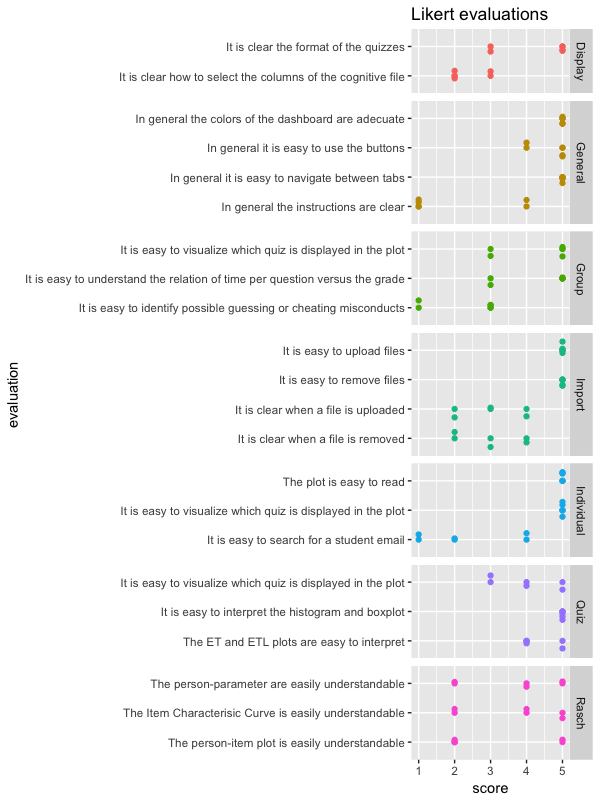
\includegraphics[width=\linewidth]{img/likert.png}
\caption{Evaluations in likert scale with a confidence interval of 1.5 standard deviation. Only 3 persons were in the focus group, then the lines are only for reference.}
\label{img:likert}
\end{figure}


From these evaluations and the commentaries from the focus group we can conclude four main points:
  
  \begin{itemize}
\item{In terms of the content in the plots, these display good and useful information} 
\item{There are some minor issues with the dashboard usability that can be improved}
\item{The rasch model should be explained in a more detailed way}
\item{The instructions shoud be more clear and detailed}
\end{itemize}

By analyzing the qualitative and the Likert evaluations, we can give more detailed areas of improvement. Concerning the lanalytics package, the majority of the plots were useful, but some suggestions were given to improve them. Some of them were as put some filters or additional characteristics, like being able to display more students in the same graph. 

For the user interface evaluations, useful insights were given. There are tabs where it is not intuitive what to do (in special the box related to the cognitive file import and the buttons to upload files) and some instructions are not clear.

For the third point, the Rasch model is a complex topic that should be explained in a much more detailed way. Currently, the instructions given in this section are not enough. Also, there should be more examples and interpretation of the parameters.

The fourth is the one that can improve a lot. It was suggested that the instructions should be more clear and explicit. Also they suggested that there should be one button that displays more detailed instructions and information. In addition it was suggested that a native English speaker proofread the dashboard in order to make the instructions clearer.






